\chapter{Testing}

\textit{Testing} is the systematic process of executing a program using data that simulates user input, aiming to ensure that the software functions as intended and meets the specified requirements.

At its core, testing serves as a methodical exploration to observe the program's behavior, providing valuable insights into its functionality. The fundamental principle guiding testing is to compare the expected behavior of the software with its actual behavior during execution. To put it simply:

\begin{itemize}
    \item If the observed behavior aligns with what is expected, the test is deemed successful.
    \item If the observed behavior deviates from expectations, the test is considered unsuccessful or failed.
\end{itemize}

\noindent Some types of testing are:

\begin{itemize}
    \item \textbf{Functional testing}: Functional testing assesses whether a software application performs its functions as expected. It involves evaluating the individual features and functionalities of the software to ensure that they conform to the specified requirements. This type of testing focuses on inputs, outputs, and the \textit{overall behavior of the system} under various conditions.
    \item \textbf{User testing}: User testing, also known as usability testing, focuses on evaluating the software from an end-user perspective. It aims to validate that the application is user-friendly, intuitive, and \textit{meets the needs of its intended users}. This type of testing often involves real users interacting with the system to identify any usability issues, design flaws, or areas for improvement in the user experience.
    \item \textbf{Performance and load testing}: Performance testing assesses the responsiveness, speed, and \textit{overall efficiency} of a software application under varying conditions. Load testing, a subset of performance testing, evaluates how the system behaves when subjected to simulated or expected levels of concurrent user activity. These tests help identify bottlenecks, measure system scalability, and ensure the software performs optimally under \textit{different workloads}.
    \item \textbf{Security testing}: Security testing focuses on identifying vulnerabilities and weaknesses within a software system to \textit{safeguard it from potential threats and unauthorized access}. This type of testing encompasses various techniques to assess the application's resistance to attacks, data breaches, and unauthorized manipulation. Security testing helps ensure that sensitive information is protected and that the software adheres to established security standards and practices.
\end{itemize}

Note that program testing can be used to show the presence of bugs, but never to show their absence: software testing will not substitute \textit{software verification}. The rest of the chapter will discuss \textbf{Functional testing} and \textbf{Security testing} in more detail.
    
\section{Functional testing}

%make it wrapped!
\begin{wrapfigure}{r}{0.3\textwidth}
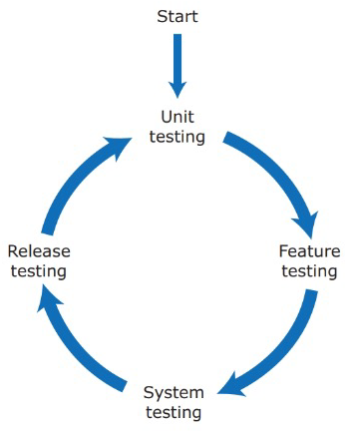
\includegraphics[width=0.3\textwidth]{images/Testing/functional-testing.png}
    \caption{Functional testing life cycle}
    \label{fig:functional-testing}
\end{wrapfigure}

Functional testing is a comprehensive set of program tests that ensure all the code is executed at least once to test the overall behavior of the system. Testing should start on the day developers begin writing code. The \textit{develop and test} cycle is simplified by automated tests. When we say that functional testing is a \textbf{staged activity}, it means that the testing process is organized and conducted in distinct stages or phases (see Figure \ref{fig:functional-testing}). It's important to note that these stages are not strictly linear and often overlap. Additionally, \textbf{regression testing} is an ongoing process that may be performed at each stage to ensure that new changes or features do not introduce defects into previously tested functionality. The division into these stages helps systematically identify and address issues at different levels of the software development cycle.

\subsection{Unit testing}

The goal of unit testing is to test program units (e.g., function, method) in \textbf{isolation}. The following is the unit test principle: \emph{If a program unit behaves as expected for a set of inputs that have some shared characteristics, it will behave the same way for a larger set whose members share these characteristics} \footnote{Example: if a program behaves correctly on the input set {1, 5, 17, 45, 99}, it is possible to conclude that it will also process all other integers in the range 1 to 99 correctly.}.

It's important to identify \textbf{equivalence partitions}: sets of inputs that will be treated the same in a code fragment, and then test the program using several inputs from each equivalence partition. Programmers usually make mistakes when defining boundaries, which is why it's recommended to use those boundaries as input for that partition. Some unit test guidelines are:

\begin{itemize}
	\item \textit{Test edge cases}: If your partition has upper and lower bounds (e.g., length of strings, numbers, etc.), choose inputs at the edges of the range.
	\item \textit{Force errors}: Choose test inputs that force the system to generate all error messages. Choose test inputs that should generate invalid outputs.
	\item \textit{Fill buffers}: Choose test inputs that cause all input buffers to overflow.
	\item \textit{Repeat yourself}: Repeat the same test input or series of inputs several times.
	\item \textit{Overflow and underflow}: If your program performs numeric calculations, choose test inputs that can cause it to calculate very large or very small numbers.
	\item \textit{Don't forget null and zero}: If your program uses pointers or strings, always test with null pointers and strings. If you use sequences, test with an empty sequence. For numeric inputs, always test with zero.
	\item \textit{Keep count}: When dealing with lists and list transformations, keep count of the number of elements in each list and check that these are consistent after each transformation.
	\item \textit{One is different}: If your program deals with sequences, always test with sequences that have a single value.
\end{itemize}

\subsection{Feature testing}

Knowing that a \textit{product feature} implements some useful user functionality, the goal of feature testing is to test that a functionality \textit{is implemented as expected} and \textit{meets the real needs of users}. Since features are normally implemented by multiple interacting program units, there are two types of tests:

\begin{itemize}
 \item \textbf{Interaction tests}: Testing interactions between units (developed usually by different developers). This type of test can also reveal bugs in program units that were not exposed by unit testing.
 \item \textbf{Usefulness tests}: Testing that a feature implements what users are likely to want. The \textit{Product manager} should be involved in designing usefulness tests.
\end{itemize}

To generate feature tests, developers must \textbf{create them from scenarios or user stories} (e.g., from user story to test: User registration: As a user, I want to be able to log in without creating a new account so that I don't have to remember another login ID and password. $\rightarrow$ Initial login screen: Test that the screen displaying a request for Google account credentials is correctly displayed when a user clicks on the ``Sign in with Google'' link. Test that the login is completed if the user is already logged in to Google.).

\subsection{System Testing}

The goal of system testing is to test the system as a whole, in order to:

\begin{itemize}
	\item Discover unexpected/unwanted interactions between the features.
	\item Discover if system features work together effectively to support what users really want to do.
	\item Ensure the system operates as expected in the different environments where it will be used.
	\item Test responsiveness, throughput, security, and other quality attributes.
\end{itemize}

One piece of advice for generating system testing is to use a set of scenarios and user stories to identify users’ end-to-end pathways since we want to test data flow across different modules.

\subsection{Release Testing}

The goal of release testing is to test a system that is intended for release to customers. Release testing tests the system in its real operational environment (rather than in a test environment). The aim is to decide if \textbf{the system is good enough to release}, not to detect bugs in the system. This type of testing is necessary because preparing a system for release involves packaging the system for deployment, installing required software and libraries, configuring parameters (and mistakes can be made in that process). If the software is deployed on the cloud, an automated continuous release process can be used.

\section{Security Testing}

Objectives of security testing are to \textbf{find vulnerabilities} that an attacker may exploit, and to \textbf{provide convincing evidence} that a system is \textbf{sufficiently secure}. Finding vulnerabilities is harder than finding bugs, as developers must test for something the software should NOT do (potentially an infinite number of tests). Normal functional tests may not reveal vulnerabilities, and the software stack (OS, libraries, databases, and so on) on which a product depends may contain vulnerabilities.

Comprehensive security testing requires specialist knowledge (e.g., involve external specialists for penetration testing, which is expensive). Usually, companies adopt a \textbf{risk-based approach} by identifying the main security risks to a product and developing tests to demonstrate that the product protects itself from these risks. \newpage \noindent It is possible to automate some of these tests, but others inevitably require manual checking of behavior and files.

\noindent Here are some examples of security risks:
\begin{itemize}
    \item An unauthorized attacker gains access to a system using authorized credentials.
    \item An authorized individual accesses resources that are forbidden to that person.
    \item The authentication system fails to detect an unauthorized attacker.
    \item An attacker gains access to the database using an SQL injection attack.
    \item Improper management of HTTP sessions.
    \item HTTP session cookies are revealed to an attacker.
    \item Confidential data are unencrypted.
    \item Encryption keys are leaked to a potential attacker.
\end{itemize}

When testing security, developers need to think like an attacker rather than a normal end-user, deliberately trying to do the wrong thing and repeating actions multiple times.

\section{Test Automation}

Automated testing is widely used in product development companies, as manual system testing is tedious and error-prone. Executable tests check that software returns the expected result for input data, as shown in Figure \ref{fig:test-runner}.

\noindent A good practice is to structure automated tests into three parts:

\begin{enumerate}
    \item \textit{Arrange}: Set up the system to run the test (define test parameters).
    \item \textit{Action}: Call the unit that is being tested with the test parameters.
    \item \textit{Assert}: Assert what should hold if the test is executed successfully.
\end{enumerate}

\begin{figure} [H]
    \centering
    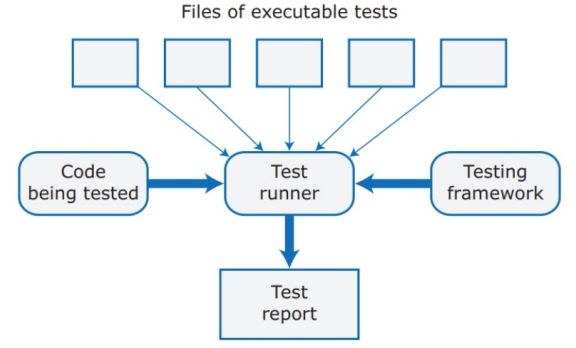
\includegraphics[width=0.63\textwidth]{images/Testing/test-runner.PNG}
    \caption{Test runner scheme}
    \label{fig:test-runner}
\end{figure} 

\textbf{Testing frameworks} are available for all widely used programming languages, so developers are free to use their code. Test code used for testing \emph{can include bugs}. Good practices to reduce the chances of test errors are to make tests as simple as possible and review all tests along with the code they test.

Unit tests are the easiest to automate. Good unit tests reduce (but do not eliminate) the need for feature tests, which is beneficial because GUI-based testing is expensive to automate (see an example in Figure \ref{fig:interaction-replicater}), while API-based testing is preferable. It is necessary to perform multiple assertions to check that the feature executed as expected.

\begin{figure} [H]
    \centering
    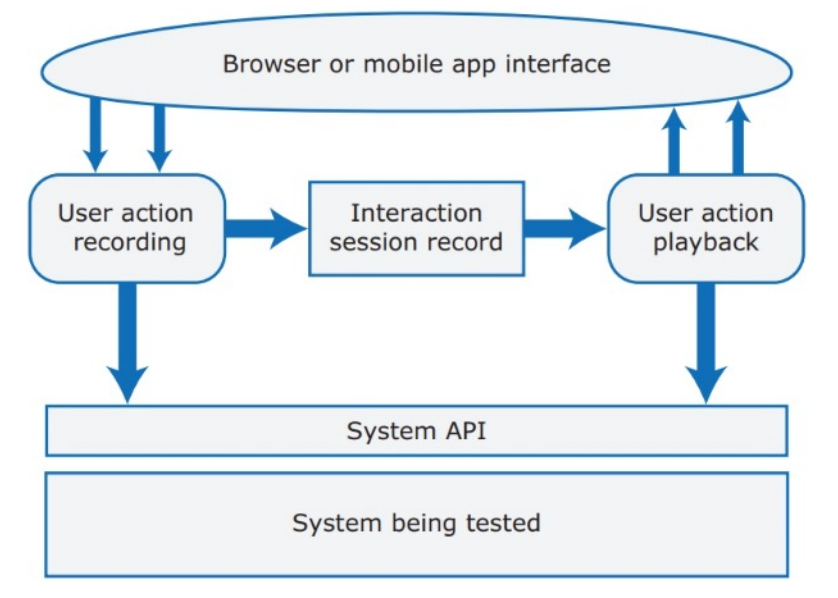
\includegraphics[width=0.65\textwidth]{images/Testing/interaction-replicater.PNG}
    \caption{GUI-based testing cycle}
    \label{fig:interaction-replicater}
\end{figure} 

\section{Test-Driven Development}

There are some Agile frameworks, such as \textit{Extreme Programming}, that are test-driven, meaning that developers must first write executable tests and then write the code to pass the tests. Figure \ref{fig:test-driven-development} shows how test-driven development can be incorporated within the development cycle. \\

\noindent Let's analyze the pros of this technique:

\begin{itemize}
    \item Systematic approach: Tests are clearly linked to code sections, so there are no untested sections.
    \item Tests help in understanding program code.
    \item Simplified, incremental debugging.
    \item Simpler code (this last point is arguable).
\end{itemize}

\begin{figure} [H]
    \centering
    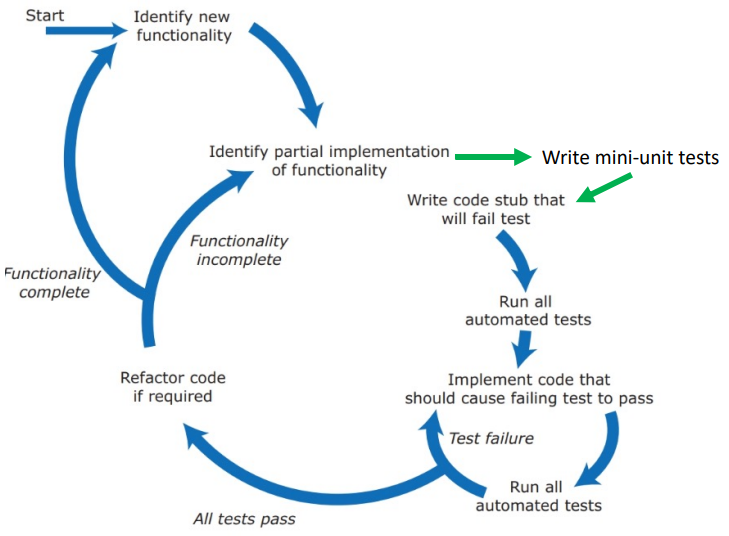
\includegraphics[width=1\textwidth]{images/Testing/test-driven-development.PNG}
    \caption{Test-driven development cycle}
    \label{fig:test-driven-development}
\end{figure} 

\noindent Let's also analyze the cons of this technique:

\begin{itemize}
    \item Difficult to apply TDD\footnote{TDD: Test-driven development} to system testing.
    \item TDD discourages radical program changes.
    \item TDD leads developers to focus on the tests rather than on the problem they are trying to solve.
    \item TDD leads developers to think too much about implementation details rather than overall program structure.
    \item Hard to write “bad data” tests.
\end{itemize}

\newpage

\section{Code Reviews}

Testing has some limitations:

\begin{itemize}
    \item Developers test code against their understanding of what that code should do. If you have misunderstood the purpose of the code, then this will be reflected in both the code and the tests.
    \item Testing may not provide coverage of all the code you have written (TDD shifts the problem to code incompleteness).
    \item Testing does not really provide insights into other attributes of a program (e.g., readability, structure, evolvability).
\end{itemize}

\noindent That's why \textbf{code reviews} complement testing. Figure \ref{fig:reviewer} shows how a \textbf{Reviewer} works.

\begin{figure} [H]
    \centering
    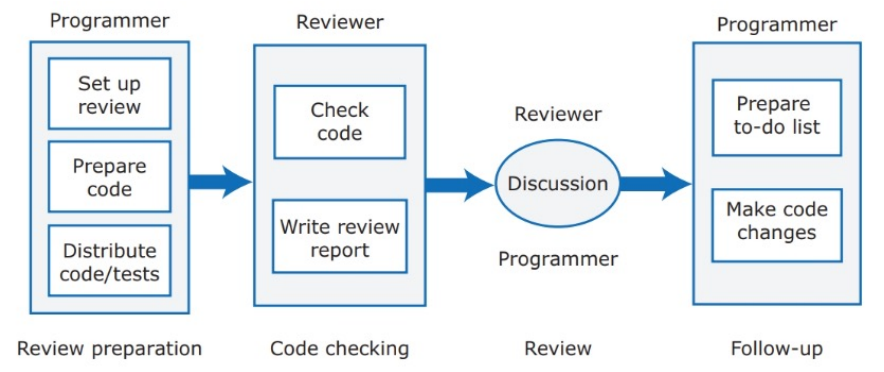
\includegraphics[width=0.8\textwidth]{images/Testing/reviewer.PNG}
    \caption{Code reviews cycle}
    \label{fig:reviewer}
\end{figure} 

Often, a single code reviewer is used (from the same DevOps team or otherwise). The reviewer can also comment on the readability and understandability of the code. Review sessions should focus on 200-400 lines of code and can be triggered by commits to shared repositories.

A checklist is often used by the reviewer to check common (or language-specific) points about the new section. Some examples are:
\begin{itemize}
    \item (General) Are meaningful variable and function names used?
    \item (General) Have all data errors been considered and tests developed for these?
    \item (General) Are all exceptions explicitly handled?
    \item (Python) Are default function parameters used?
    \item (Python) Are types used consistently?
    \item (Python) Is the indentation level correct?
\end{itemize}
